\appendix

\chapter{Source Code}

The following code was used to manage, analyze, and graph output results from CH Instruments 1207 and 660B potentiostats that had been converted to text. It supports cyclic voltammetry, amperometry, and differential pulse voltammetry files. It is written for Python 2.5 and uses the Django package. Included here are only the files that perform management, analysis, and graphing. It is available in its entirety online at http://github.com/mjibson/biosensor/.

\singlespacing
\lstset{language=Python,basicstyle=\tiny,breaklines,tabsize=2}

biosensor/models.py:
\lstinputlisting{verbatim/biosensor/models.py}

biosensor/plot.awk:
\lstinputlisting{verbatim/biosensor/plot.awk}

biosensor/views.py:
\lstinputlisting{verbatim/biosensor/views.py}

\chapter{Screenshots}

The following screenshots are selected from the application described above.

\begin{figure}
	\centering
	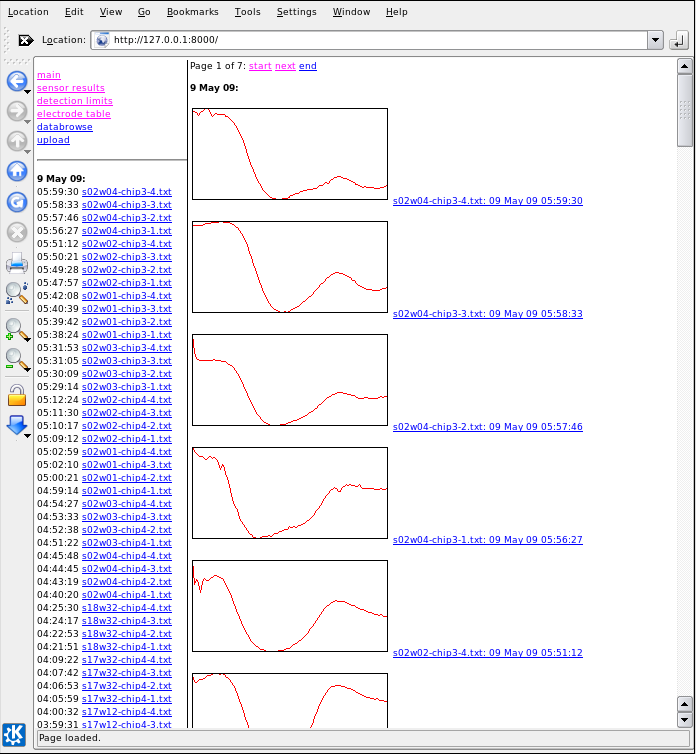
\includegraphics[width=\linewidth]{figures/web-main.png}
	\caption{Web application main page}
\end{figure}

\begin{figure}
	\centering
	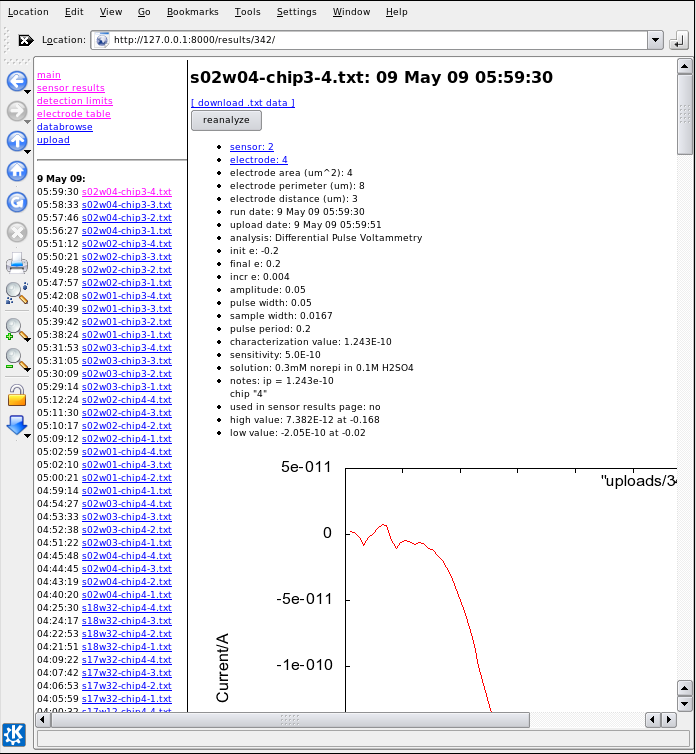
\includegraphics[width=\linewidth]{figures/web-detail.png}
	\caption{Web application result detail}
\end{figure}

\begin{figure}
	\centering
	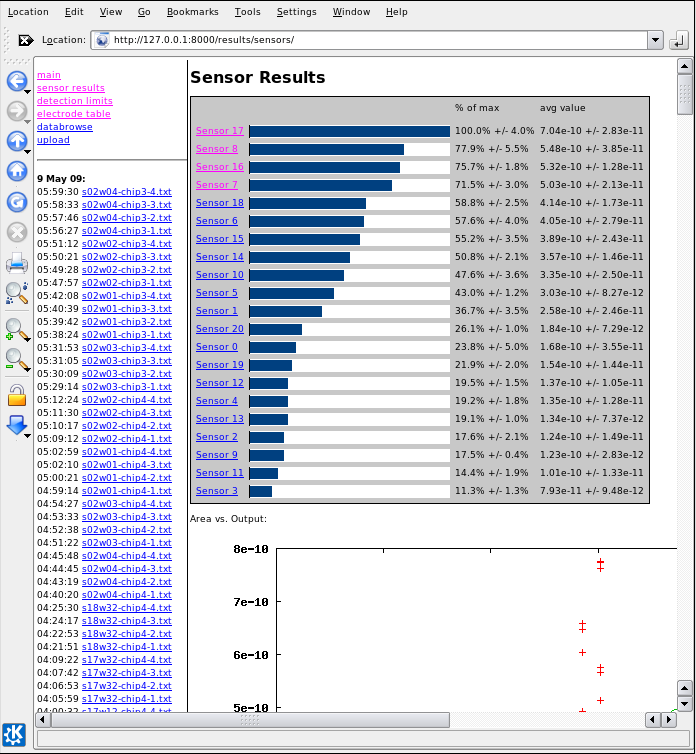
\includegraphics[width=\linewidth]{figures/web-sensors.png}
	\caption{Web application sensor results}
\end{figure}

\begin{figure}
	\centering
	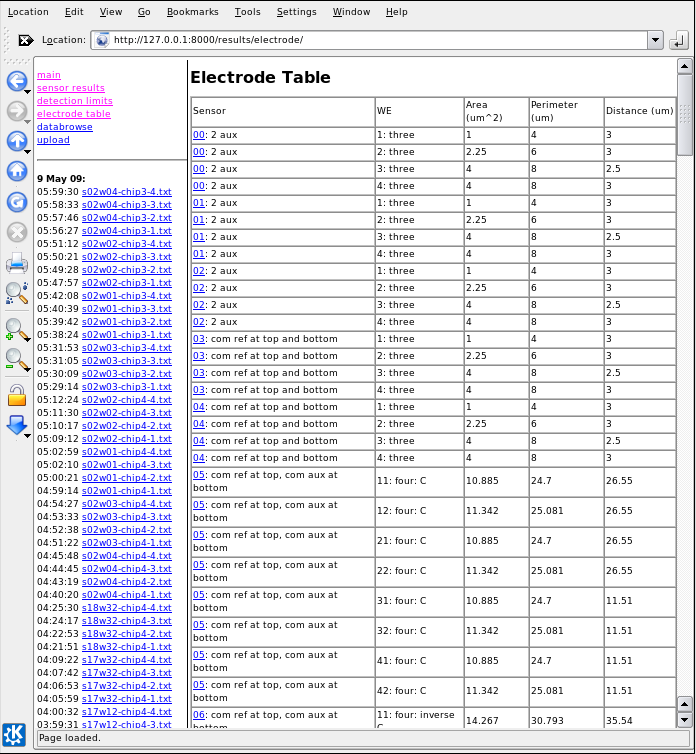
\includegraphics[width=\linewidth]{figures/web-electrodes.png}
	\caption{Web application electrode table}
\end{figure}

\chapter{Solution Mixing}

This chapter describes the process for mixing the solutions used during testing. If the desired solution is $20 \mathrm{mL}$ of $0.3 \mathrm{mM}$ norepinephrine in $0.1 \mathrm{M}$ $\mathrm{H}_2 \mathrm{SO}_4$:
\begin{enumerate}
	\item Measure the correct amount of norepinephrine (labeled as arterenol in the chemistry lab) by finding its molecular weight, listed on the vial, which is $319.3 \mathrm{g/mol}$. Multiply the weight, desired solution amount, and desired molarity together:
		\begin{displaymath}
			0.3 \mathrm{mM} * 319.3 \mathrm{g/mol} * 20 \mathrm{mL} = 0.00192 \mathrm{g}
		\end{displaymath}
		Hence, measure $0.00192 \mathrm{g}$ of norepinephrine, and put it in a vial.
	\item Create your $0.1 \mathrm{M}$ $\mathrm{H}_2 \mathrm{SO}_4$ solution by first determining how much distilled water is needed. Find the molarity of $\mathrm{H}_2 \mathrm{SO}_4$, which is $18.4 \mathrm{M}$. Divide the product of the desired final molarity and the desired volume by that molarity:
		\begin{displaymath}
			(0.1 \mathrm{M} * 20 \mathrm{mL}) / 18.4 \mathrm{M} = 0.1087 \mathrm{mL}
		\end{displaymath}
		Hence, $0.1087 \mathrm{mL}$ is the amount of $\mathrm{H}_2 \mathrm{SO}_4$ needed to make $20 \mathrm{mL}$ of $0.1 \mathrm{M}$ $\mathrm{H}_2 \mathrm{SO}_4$.
	\item Add the appropriate amount of distilled water to the vial with the norepinephrine. Since we are getting $20 \mathrm{mL}$, subtract the number found in the previous step, and add that much distilled water:
		\begin{displaymath}
			20 \mathrm{mL} - 0.1087 \mathrm{mL} = 19.89 \mathrm{mL}
		\end{displaymath}
		Hence, add $19.89 \mathrm{mL}$ of distilled water to the vial. Always add the water first. Do not add the acid before the water.
	\item Now, after adding the water, add the acid. Add $0.1087 \mathrm{mL}$ of $\mathrm{H}_2 \mathrm{SO}_4$ to the vial.
\end{enumerate}

You should now have $20 \mathrm{mL}$ of $0.3 \mathrm{mM}$ norepinephrine in $0.1 \mathrm{M}$ $\mathrm{H}_2 \mathrm{SO}_4$. It will last a few days before degrading to an unusable point. If kept in a fridge it will last longer.
